\documentclass[border=4pt]{standalone}
\usepackage{tikz}
\usetikzlibrary{arrows.meta,calc,shapes.geometric}
\begin{document}
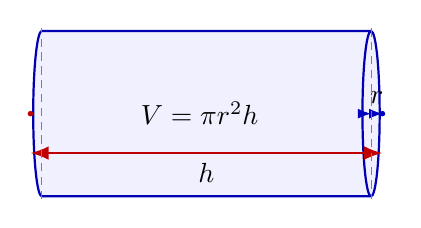
\begin{tikzpicture}[>=Latex]
  \node[cylinder,shape aspect=.42,draw=blue!70!black,thick,fill=blue!6,
    minimum width=21mm,minimum height=44mm,outer sep=1pt] (solid)
    {$V=\pi r^2h$};

  \draw[<->,red!75!black,thick]
    ($(solid.bottom)+(0,-5mm)$) --
    node[below,black] {$h$}
    ($(solid.top)+(0,-5mm)$);
  \coordinate (cap center) at ($(solid.before top)!0.5!(solid.after top)$);
  \draw[<->,blue!75!black]
    (cap center) -- node[above,black] {$r$} (solid.top);
  \draw[densely dashed,gray] (solid.before bottom) -- (solid.after bottom);
  \draw[densely dashed,gray] (solid.before top) -- (solid.after top);
  \fill[blue!75!black] (solid.top) circle (1pt);
  \fill[red!75!black] (solid.bottom) circle (1pt);
\end{tikzpicture}
\end{document}
